%% 
%% Copyright 2019-2021 Elsevier Ltd
%% 
%% This file is part of the 'CAS Bundle'.
%% --------------------------------------
%% 
%% It may be distributed under the conditions of the LaTeX Project Public
%% License, either version 1.2 of this license or (at your option) any
%% later version.  The latest version of this license is in
%%    http://www.latex-project.org/lppl.txt
%% and version 1.2 or later is part of all distributions of LaTeX
%% version 1999/12/01 or later.
%% 
%% The list of all files belonging to the 'CAS Bundle' is
%% given in the file `manifest.txt'.
%% 
%% Template article for cas-dc documentclass for 
%% double column output.

\documentclass[a4paper,fleqn]{cas-dc}

% If the frontmatter runs over more than one page
% use the longmktitle option.

%\documentclass[a4paper,fleqn,longmktitle]{cas-dc}

% \usepackage[numbers]{natbib}
\usepackage[authoryear]{natbib}
% \usepackage[authoryear,longnamesfirst]{natbib}

\usepackage{hyperref}
\hypersetup{
    % colorlinks = false, % default value = true; used during formatting
    % allcolors = {teal}, % color used while writing, recommanded if within guidelines
    allcolors = {black}, % consistent look
}
\usepackage{cleveref}

%%%Author macros
\def\tsc#1{\csdef{#1}{\textsc{\lowercase{#1}}\xspace}}
\tsc{WGM}
\tsc{QE}
%%%

% Uncomment and use as if needed
%\newtheorem{theorem}{Theorem}
%\newtheorem{lemma}[theorem]{Lemma}
%\newdefinition{rmk}{Remark}
%\newproof{pf}{Proof}
%\newproof{pot}{Proof of Theorem \ref{thm}}


\begin{document}
\let\WriteBookmarks\relax
\def\floatpagepagefraction{1}
\def\textpagefraction{.001}

% Short title
% \shorttitle{<short title of the paper for running head>}    
\shorttitle{Design paper for a novel approach to the machine learning system in the healthcare industry.}

% Short author
% \shortauthors{<short author list for running head>}  
\shortauthors{Ketkar Y., Gawade S.}

% Main title of the paper
\title [mode = title]{Design paper for a novel approach to the machine learning system in the healthcare industry.}

\let\printorcid\relax

% Title footnote mark
% eg: \tnotemark[1]
% \tnotemark[<tnote number>] 

% Title footnote 1.
% eg: \tnotetext[1]{Title footnote text}
% \tnotetext[<tnote number>]{<tnote text>} 

% First author
%
% Options: Use if required
% eg: \author[1,3]{Author Name}[type=editor,
%       style=chinese,
%       auid=000,
%       bioid=1,
%       prefix=Sir,
%       orcid=0000-0000-0000-0000,
%       facebook=<facebook id>,
%       twitter=<twitter id>,
%       linkedin=<linkedin id>,
%       gplus=<gplus id>]

\author[1]{Yashodhan Ketkar}

% Corresponding author indication
% \cormark[<corr mark no>]

% Footnote of the first author
% \fnmark[<footnote mark no>]

% Email id of the first author
\ead{ketkaryapr19me@student.mes.ac.in}

% URL of the first author
% \ead[url]{<URL>}

% Credit authorship
% eg: \credit{Conceptualization of this study, Methodology, Software}
% \credit{<Credit authorship details>}

% Address/affiliation
\affiliation[1]{organization={Department of Information Technology Engineering, Pillai College of Engineering},
    % addressline={}, 
    city={New Panvel},
    % citysep={}, % Uncomment if no comma needed between city and postcode
    postcode={410206},
    % state={Maharashtra},
    country={India}}

\author[2]{Sushopti Gawade}

% Footnote of the second author
% \fnmark[2]

% Email id of the second author
\ead{sgawade@mes.ac.in}

% URL of the second author
% \ead[url]{}

% Credit authorship
% \credit{}

% Address/affiliation
\affiliation[2]{organization={Department of Computer Engineering, Pillai College of Engineering},
    % addressline={}, 
    city={New Panvel},
    %          citysep={}, % Uncomment if no comma needed between city and postcode
    postcode={410206},
    % state={Maharashtra},
    country={India}}

% Corresponding author text
% \cortext[2]{Corresponding author}

% Footnote text
% \fntext[1]{}

% For a title note without a number/mark
%\nonumnote{}

% Here goes the abstract
\begin{abstract}
    The use of machine learning in various fields is still limited. The driving reason behind this is the lack of ease-to-use systems for non-technical people. The objective of this paper is to provide the general population access to a machine learning system. We propose an automated machine learning system for non-technical users. The proposed system automates the selection of the best model as per user requirements. We employed the proposed system on Parkinson's disease datasets in this study. The proposed system showed high accuracy in training the machine learning models and the selection of appropriate models as per user requirements. As per tests conducted the proposed system showed satisfactory performance.
\end{abstract}

% Use if graphical abstract is present
%\begin{graphicalabstract}
%\includegraphics{}
%\end{graphicalabstract}

% Research highlights
% \begin{highlights}
% \item a
% \item a
% \item a
% \end{highlights}

% Keywords
% Each keyword is seperated by \sep
\begin{keywords}
   Automated Selection System \sep 
   General Prediction System \sep
   Healthcare Industry \sep
   Parkinson's Disease Detection \sep
   Supervised Learning Algorithms
\end{keywords}

% \tolerance 9999
% \hbadness=10000

\maketitle


% Main text
% \section{Introduction}\label{sec:introduction}
\section{Introduction} \label{sec:introduction}

COVID-19 has been widespread in recent years. It targets the human respiratory system, causing severe respiratory issues. Depending on a person's condition and the prevalence of comorbidities, this disease can be fatal. Cardiovascular comorbidities are frequent in COVID-19 disease. Cardiovascular comorbidities are also problematic to diagnose in the absence of suitable equipment. Checking for arrhythmia in patients is one approach to detection. Arrhythmia is the irregular beating of the heart. Arrhythmia is detected by examining ECG signals. Because COVID-19 has put a strain on the medical personnel, detection takes longer than usual. Increased Internet connectivity has led to the use of machine learning and artificial intelligence (AI) for service in a variety of sectors. This increases research in the field of machine learning and has an impact on machine learning in a variety of domains. One of them is the medical and healthcare businesses. Machine learning is used to detect and categorize viruses and other microorganisms in patients. In medical applications, machine learning algorithms have already been shown to be quite useful.

The machine learning system may be used to scan these ECG signals and detect them. These signs may be detected considerably faster and more efficiently using supervised learning techniques. In such exact classification problems, supervised algorithms have previously been demonstrated to be quicker than unsupervised techniques. Once taught, this algorithm may also be utilized to make future predictions.

There are several supervised algorithms accessible, allowing us to select the best method for our purposes. This phase can be automated in the case of the general population. A few methods may be pre-programmed into the system, and the computer can then train and pick the best model for the supplied dataset. This will free up medical personnel to focus on patient care and problem-solving.

\section{Literature Review} \label{sec:literature_review}

\cite*{02_rp} suggest that arrhythmia is one of the most common symptoms in patients with COVID19. {\responsemod Arrhythmia was found in 7\% of all Wuhan COVID-19 cases and 14.8\% of patients with poor outcomes.} \cite*{18_rp} state that 17\% of patients hospitalized in China were diagnosed with arrhythmia. \citeauthor{18_rp} conducted a review of 10 eligible studies (5,193 patients) for analysis and found that atrial arrhythmia was present in 9.2\% of cases. A review by \cite*{15_rp} of 17 studies with 5,815 patients showed that arrhythmia was detected in 9.3\% of COVID-19 cases. \cite*{25_rp} suggest that only 8\% of patients with arrhythmia had prior cardiovascular conditions. {\responsemod \citeauthor{25_rp} also mentioned that 56\% of patients showed symptoms after the COVID-19 infection.}

\cite*{24_rp} used an ensemble classifier to detect the anomalies in the ECG signal. This approach, which combines multiple classifiers for prediction, has proven effective because the accuracy of the ensemble classifier is significantly higher than that of a single classifier. A few authors used this approach to improve the prediction accuracy of supervised learning models. \cite*{10_rp} used the maximal overlap wavelet packet transform ensemble with a neural network and achieved satisfactory results. \cite*{20_rp} used the ensemble approach to predict the results of the students. \citeauthor{20_rp} state the model was able to predict the correct results even with a small amount of training data. \cite*{16_rp} compared the FLINK-based iForest ensembled algorithms against the sklearn-iForset and other algorithms. \citeauthor{16_rp} concluded that the Flink-iForest algorithm showed better performance than off-the-shelf algorithms. \cite*{11_rp} used the AutoML algorithm and tools on data streams. \citeauthor{11_rp} concluded that the default classifiers can be used with AutoML tools for accurate prediction. With AutoML tools, prediction systems can be automated.

\cite*{ref_paper_m1} used machine learning for the prediction of end-of-semester results. \cite*{ref_paper_m1} used SVM, KNN, and DT models. \cite*{ref_paper_m1} concluded that the machine learning system performed satisfactorily, with SVM achieving up to 78\% accuracy.

\cite*{23_rp} extracted appropriate features for the detection of epileptic seizures. \citeauthor{23_rp} preprocessed data and used ML algorithms on the data. \citeauthor{23_rp} concluded that the supervised learning models showed more effectiveness than the unsupervised learning models. \cite*{12_rp} used a commercial classifier for the detection of arrhythmia. \citeauthor{12_rp} used ECG signals from patients and applied a custom SVM classifier. \citeauthor{12_rp} concluded that the algorithm was a successful and efficient {\responsemod detector} of arrhythmia.

\cite*{ref_paper_m2} used supervised learning algorithms for the early detection of heart disease and diabetes disease. \cite*{ref_paper_m2} concluded that the model performed satisfactorily.

\cite*{09_rp} used neural networks to process raw ECG signals and make predictions. {\responsemod While \cite*{22_rp} used small neural networks for efficient recognition processes, both studies concluded that artificial neural networks are extremely efficient and accurate in the prediction of anomalies.}

\cite*{06_rp} showed that the LDA classifier can outperform the SVM classifier in low-performance environments and lightweight systems. The self-learning algorithm makes the system more dynamic and adaptable to incoming signals. \cite*{14_rp} used adaptive fuzzy algorithms to classify ECG signals. \citeauthor{14_rp} stated that the algorithm showed satisfactory results, but it requires {\responsemod prior} classification patterns results. \cite*{ref_paper_self_rpa} suggest that the RPA system can be used in these systems for easier integration of machine learning with dynamic data. \cite*{21_rp} used ECG signals of COVID-19 patients for patient monitoring. \citeauthor{21_rp} used LSTM, SVM, and MLP algorithms to monitor data. \citeauthor{21_rp} suggest that machine learning with robotics can provide better results.

\cite*{07_rp} used a multi perceptron neural network for stroke predictions. The neural network showed high accuracy. \citeauthor{07_rp} were able to achieve up to 78\% accuracy. \citeauthor{07_rp} suggest that the model can produce better results with a larger training dataset. \cite*{05_rp} used artificial intelligence to detect heart disease. \citeauthor{05_rp} concluded that the algorithms achieved up to 83\% accuracy. \citeauthor{05_rp} also concluded that the system was able to comply with the HIPAA regulations.

\cite*{ref_paper_m3} used machine learning algorithms to predict crop growth rates. {\responsemod \citeauthor{ref_paper_m3} were able to get good insights into the field.} \citeauthor{ref_paper_m3} concluded that the use of machine learning will result in minimizing complexity and increasing yield in farming.

\cite*{01_rp} used a two-year dataset collected by Glumo Lake and used their expertise to train and select models. A mixed approach of data-driven and knowledge-driven modeling is used for the success of the application. \cite*{13_rp} used loo rate and stop criteria for model selection. \citeauthor{13_rp} investigated eight different issues and found that a larger loo rate was more desirable. \citeauthor{13_rp} also suggested that modeling difficulties can only be found by careful numerical calculations.

\cite*{17_rp} used a novel kernel to get the dataset description. \citeauthor{17_rp} concluded that this approach led to the discovery of invisible models. \citeauthor{17_rp} also state that this approach reduces the amount of human interaction. \cite*{04_rp} created a new model using the glmulti package. These models are unique and flexible. The model is automatically optimized to provide a multi-model interface. This approach allows you to quickly explore a large set of models for selection purposes. \cite*{08_rp} optimized parameters with a genetic algorithm. \citeauthor{08_rp} successfully used a genetic algorithm to reduce uncertainty in the prediction results. These methods can be used for the automated model selection system.

\section{Design and Implmentation}\label{sec:design_and_implmentation}

\subsection{System Architecture}\label{subsec:system_architecture}

The goal of the system is to be used by non-technical users. The system consists of three processes or modules. These processes are the training process, selection process, and prediction process. The first two processes interact with each other. Their task is to produce the best-suited model for the user's needs. The third process interacts with the selected models to generate the predictions. \autoref{fig:system_architecture}, shows the architecture of the system. The user is indirectly allowed to access the training and prediction process. The user data is stored on a local drive for easier and faster access.

\begin{figure}[ht]
    \centering
    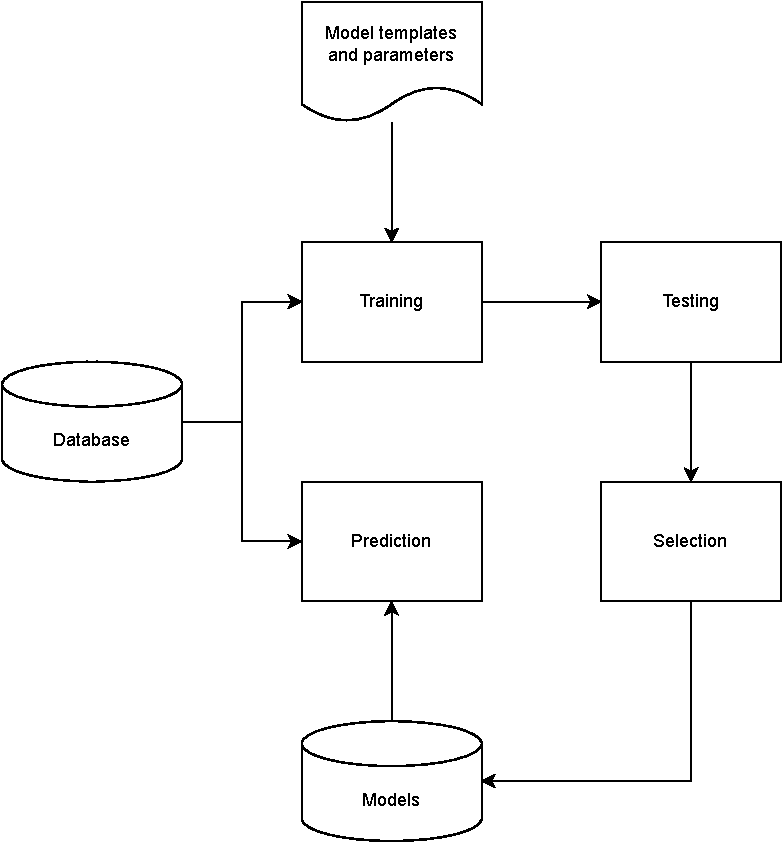
\includegraphics[width=0.9\columnwidth]{media/sec03/system_architecture.pdf}
    \caption{System Architecture}
    \label{fig:system_architecture}
\end{figure}

\subsection{System Processes}\label{subsec:system_processes}

As stated in previous section, the system consists of three primary processes. These processes are the training process, selection process, and prediction process. These processes are described in the following sections.

\subsubsection{Training Process}\label{subsubsec:training_process}

The training process is the first process in the system. \autoref{fig:training_process}, shows the structure of the training process. The training process has many functions. The first function is gathering data from the user and pre-processing it for training purposes. The training process also generates models with the template, which contains model structure and parameters. These models are trained with processed data and stored for future use. The performance of models is also calculated during this phase and store for selection purpose.

\begin{figure}[ht]
    \centering
    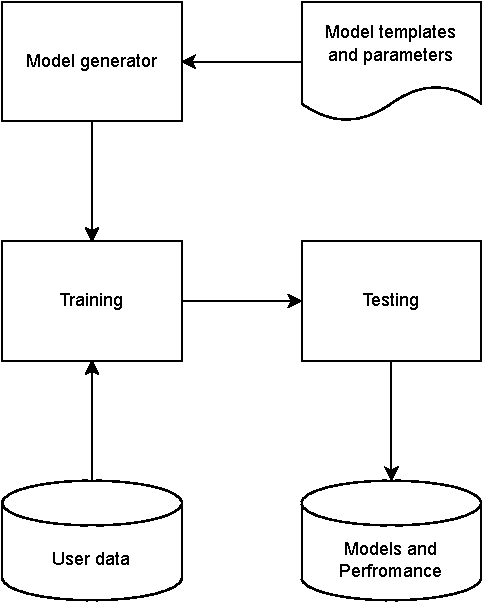
\includegraphics[width=0.6\columnwidth]{media/sec03/training_and_testing.pdf}
    \caption{Training Process}
    \label{fig:training_process}
\end{figure}

\subsubsection{Selection Process}\label{subsubsec:selection_process}

The selection process is second in the system. \autoref{fig:selection_process}, shows the structure of the training process. This process evaluates the performance of models based on metrics and weightage. The metrics of models are generated during the training process. The performance weightage is defined by the user depending on requirements. The final performance score is calculated and used for selection of the best model for users task. The selected model is stored in a separate directory with a label for easier access. This model will be used for prediction problems.

\begin{figure}[ht]
    \centering
    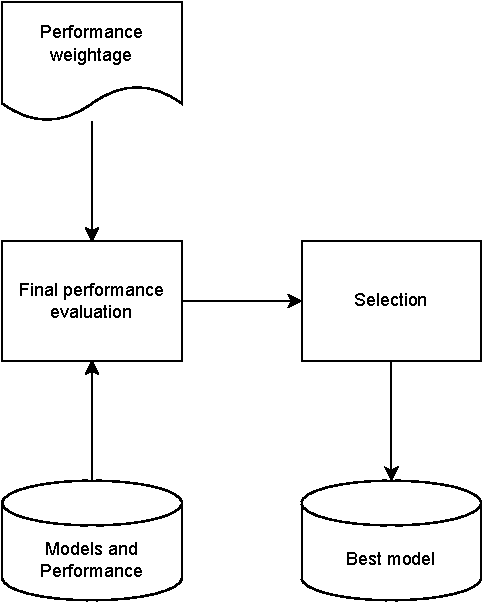
\includegraphics[width=0.6\columnwidth]{media/sec03/selection.pdf}
    \caption{Selection Process}
    \label{fig:selection_process}
\end{figure}

\subsubsection{Prediction Process}\label{subsubsec:prediction_process}

The prediction process is the final process in the system. \autoref{fig:prediction_process}, shows the structure of the prediction process. This process unpacks the best model and loads it for prediction. The model generates predictions with user-provided data. The output is displayed to the user. This output is also stored for future reference.

\begin{figure}[ht]
    \centering
    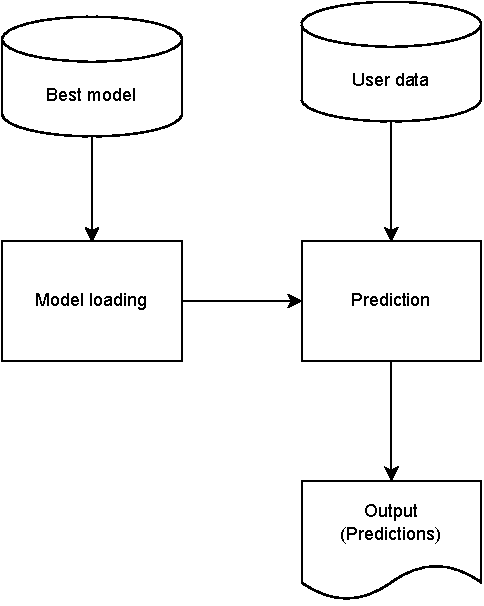
\includegraphics[width=0.6\columnwidth]{media/sec03/prediction.pdf}
    \caption{Prediction Process}
    \label{fig:prediction_process}
\end{figure}

\subsection{Algorithms}\label{subsec:algorithms}

The system uses two algorithms to run. These algorithms are training and selection algorithms and prediction algorithms.

\vspace{-0.5em}
\subsubsection*{Training and Selection Algorithm}\label{subsubsec:training_and_selection_algorithm}
\vspace{0.5em}
\begin{enumerate}
    \item Collect/Receive dataset.
    \item Split data into 80:20 ratio for training and testing.
    \item Build a model from presets.
    \item Train models with training dataset and store models.
    \item Evaluate the performance of models with the testing dataset.
    \item Rank models with help of performance and premade tuning parameters.
    \item Selects the best model and stores it for future use.
\end{enumerate}

\vspace{-0.5em}
\subsubsection*{Prediction Algorithm}\label{subsubsec:prediction_algorithm}
\vspace{0.5em}
\begin{enumerate}
    \item Collect/Receive dataset.
    \item Load best-suited model data from the storage.
    \item Unpack model for predictions.
    \item Make predictions with the provided dataset and loaded model.
    \item Return predictions to user.
\end{enumerate}

\subsection{Implmentation}\label{subsec:implmentation}

\subsubsection{Web Architecture}\label{subsubsec:web_architecture}

The system provides service with a web application. The users aren't allowed to interact with the system directly. This provision is to provide security and reduce the outside influence on results. The interface layer is used for a user to interact with the system indirectly. \autoref{fig:web_architecture}, shows the web architecture of the system. The system is connected to the database directly. A direct connection is provided to access live data. User-provided data is processed by the system and stored in the database.

\begin{figure}[ht]
    \centering
    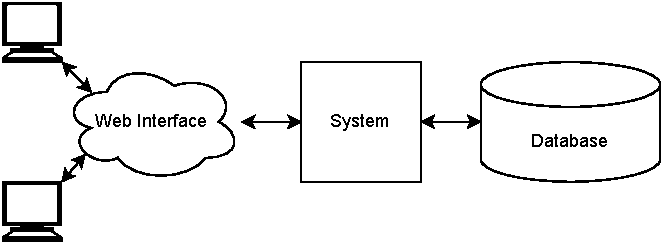
\includegraphics[width=0.9\columnwidth]{media/sec03/web_architecture.pdf}
    \caption{Web Architecture}
    \label{fig:web_architecture}
\end{figure}

\subsubsection*{Web Interface}\label{subsubsec:web_interface}
The web interface provides users with a way to interact with the system. The primary function of the web interface is to provide secure access to the system process. Approved users can interact with various modules on the system. This interface allows users to access selection and prediction processes. Users can upload data to the system.

The interface presents prediction results as well as performance evaluation results. Prediction results are provided in tabular format and stored in CSV files for future reference. Performance results are presented in graphical format and also stored in CSV files for future reference.

\section{Result and Analysis}\label{sec:result_and_analysis}

\subsection{Dataset}\label{subsec:dataset}

% To test the selection system, we used three datasets. All three datasets have very different structures. Dataset 1 [\citenum{sakar2019comparative,parkinsons_disease_classification}] contains 149 records with 23 features. Dataset 2 [\citenum{little2007exploiting,parkinsons_disease_detection}] contains 201 records with 754 features. Dataset 3 [\citenum{ecg_heartbeat}] contains 65661 records with 188 features.

% To test the selection system, we used three datasets. All three datasets have very different structures. Dataset 1 contains 149 records with 23 features [\citenum{parkinsons_disease_classification}]. Dataset 2 contains 201 records with 754 features [\citenum{parkinsons_disease_detection}]. Dataset 3 contains 65661 records with 188 features [\citenum{ecg_heartbeat}].

To test the selection system, we used three datasets. All three datasets have very different structures. Dataset 1 contains 149 records with 23 features [\citenum{parkinsons_disease_classification}]. Dataset 2 contains 201 records with 754 features [\citenum{parkinsons_disease_detection}]. Dataset 3 contains 65661 records with 188 features [\citenum{ecg_heartbeat}].

Dataset 1 is the smallest dataset with a lower number of features compared to other two datasets. Dataset 2 also contains few records, but contains the highest amount of features compared to other two datasets. While, dataset 3 has a large number of records and moderate amount of features.

\subsection{Results}\label{subsec:results}

After providing the datasets mentioned in the previous section, the system trained a few models on those datasets. The application selected the best-suited model based on datasets. 

\autoref{fig:performance_analysis_dataset_1}, shows the performance of various models trained on dataset 1. Due to the small number of records and few features model is overtrained in the case of few models. The values in \autoref{tab:performance_analysis_dataset_1}, suggest that KNN and RF models were overtrained. The KNN model is selected as the best model for this dataset.

\begin{figure}[ht]
    \centering
    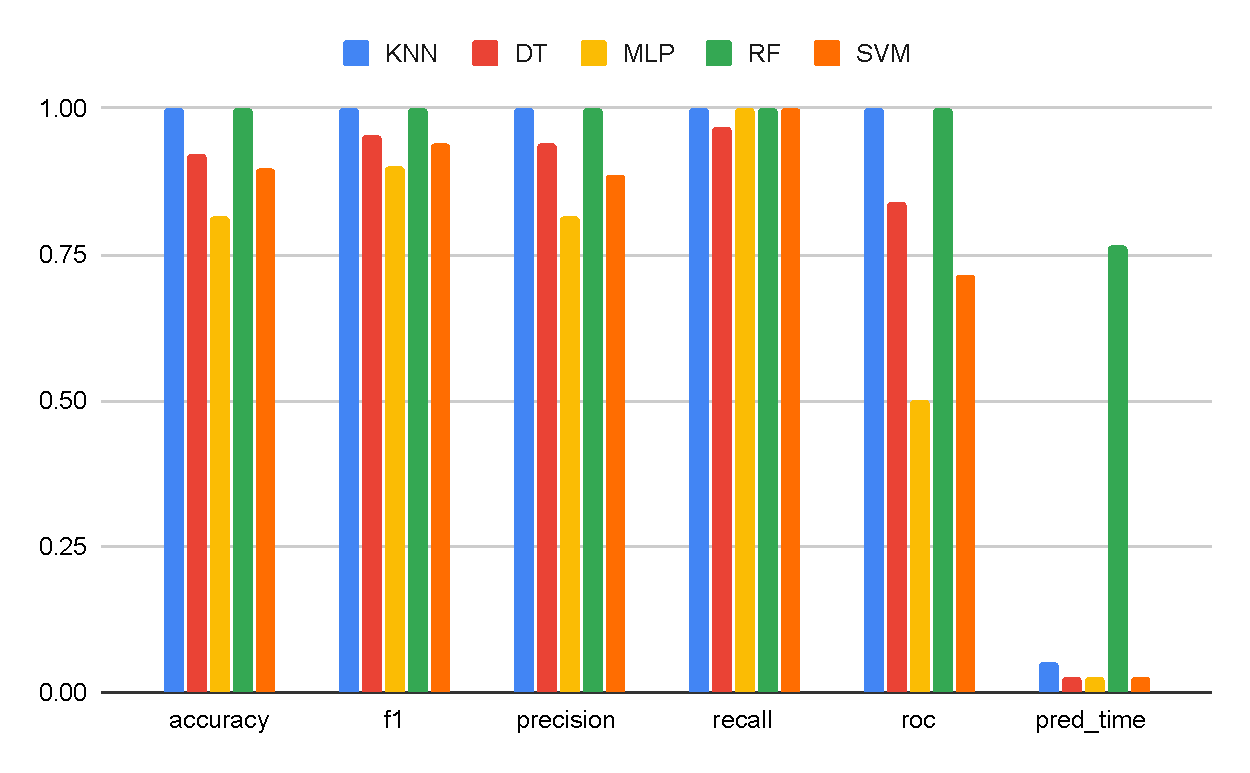
\includegraphics[width=0.9\columnwidth]{media/sec04/dataset_1_performance_evaluation.pdf}
    \caption{Performance Analysis Dataset 1}
    \label{fig:performance_analysis_dataset_1}
\end{figure}

\begin{table}[ht]
\caption{Performance Analysis of Dataset 1}\label{tab:performance_analysis_dataset_1}
\begin{tabular*}{\tblwidth}{@{}LLLLLL@{}}
\toprule
Metrics & KNN & DT & MLP & RF & SVM \\ % Table header row
\midrule
Accuracy & 1.00 & 0.92 & 0.82 & 1.00 & 0.89 \\
F1 & 1.00 & 0.95 & 0.89 & 1.00 & 0.94 \\
Pricision & 1.00 & 0.93 & 0.82 & 1.00 & 0.88 \\
Recall & 1.00 & 0.97 & 1.00 & 1.00 & 1.00 \\
ROC & 1.00 & 0.84 & 0.50 & 1.00 & 0.71 \\
Time & 0.05 & 0.02 & 0.02 & 0.76 & 0.02 \\
\bottomrule
\end{tabular*}
\end{table}

\autoref{fig:performance_analysis_dataset_2}, shows the performance of various models trained on dataset 2. This dataset also had a small number of records, but the number of features is extremely high. The values from \autoref{tab:performance_analysis_dataset_2}, shows the random forest performed better across all parameters but prediction time. The system selected the Random Forest model as best suited mode.

\begin{figure}[ht]
    \centering
    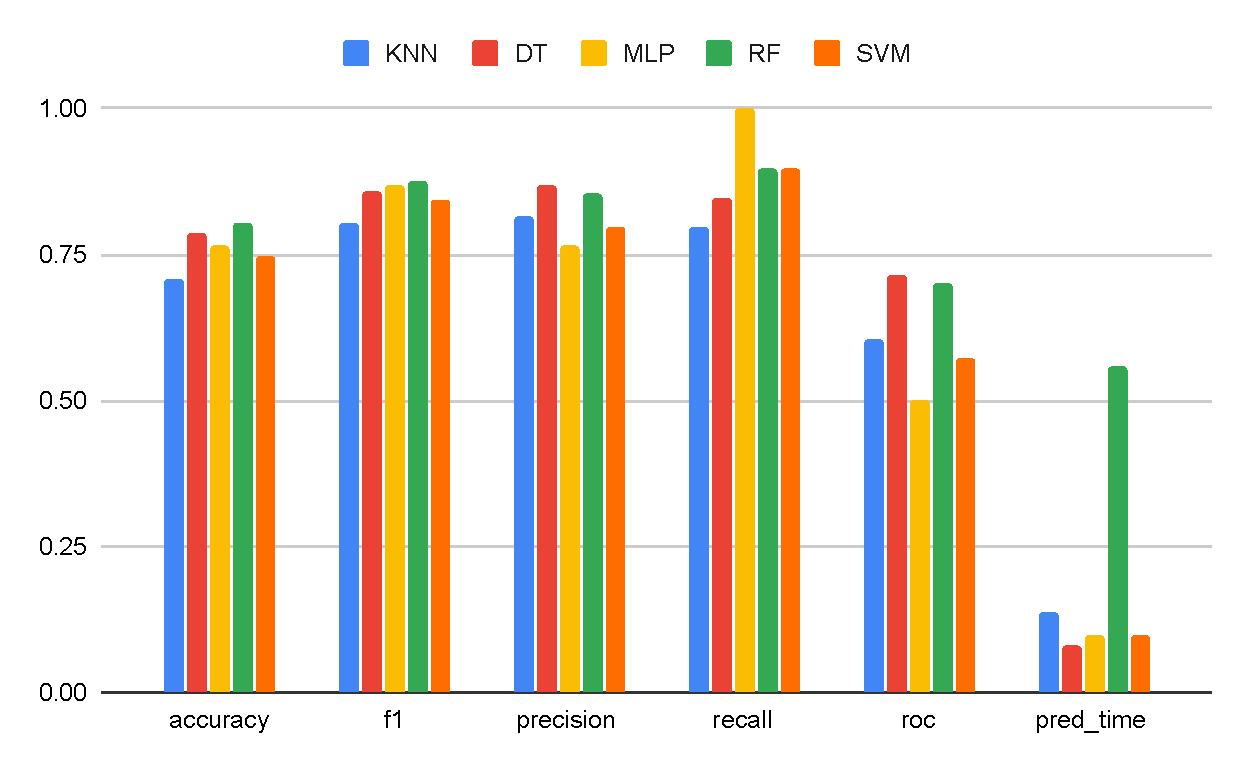
\includegraphics[width=0.9\columnwidth]{media/sec04/dataset_2_performance_evaluation.pdf}
    \caption{Performance Analysis Dataset 2}
    \label{fig:performance_analysis_dataset_2}
\end{figure}

\begin{table}[ht]
\caption{Performance Analysis of Dataset 2}\label{tab:performance_analysis_dataset_2}
\begin{tabular*}{\tblwidth}{@{}LLLLLL@{}}
\toprule
Metrics & KNN & DT & MLP & RF & SVM \\ % Table header row
\midrule
Accuracy & 0.71 & 0.78 & 0.76 & 0.80 & 0.75 \\
F1 & 0.81 & 0.86 & 0.87 & 0.88 & 0.84 \\
Precision & 0.82 & 0.67 & 0.76 & 0.85 & 0.80 \\
Recall & 0.79 & 0.85 & 1.00 & 0.90 & 0.90 \\
ROC & 0.61 & 0.71 & 0.50 & 0.70 & 0.57 \\
Time & 0.13 & 0.07 & 0.09 & 0.55 & 0.09 \\
\bottomrule
\end{tabular*}
\end{table}

\autoref{fig:performance_analysis_dataset_3}, shows the performance of various models trained on dataset 3. This dataset had a very high number of records and a moderate amount of features. The values from \autoref{fig:performance_analysis_dataset_3}, shows that almost all models performed satisfactorily on this dataset. The system selected the SVM model as best suited mode.

\begin{figure}[ht]
    \centering
    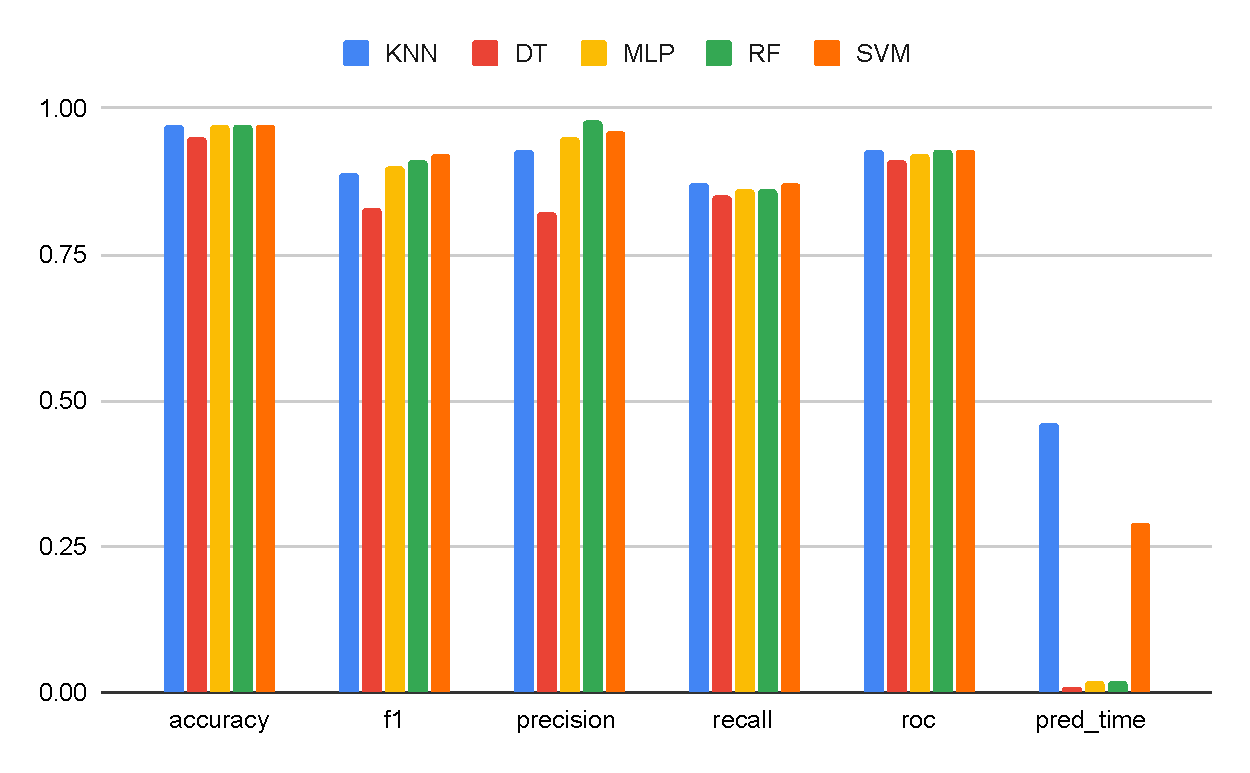
\includegraphics[width=0.9\columnwidth]{media/sec04/dataset_3_performance_evaluation.pdf}
    \caption{Performance Analysis Dataset 3}
    \label{fig:performance_analysis_dataset_3}
\end{figure}

\begin{table}[ht]
\caption{Performance Analysis of Dataset 3}\label{tab:performance_analysis_dataset_3}
\begin{tabular*}{\tblwidth}{@{}LLLLLL@{}}
\toprule
Metrics & KNN & DT & MLP & RF & SVM \\ % Table header row
\midrule
Accuracy & 0.97 & 0.95 & 0.97 & 0.97 & 0.97 \\
F1 & 0.89 & 0.83 & 0.90 & 0.91 & 0.92 \\
Precision & 0.93 & 0.82 & 0.95 & 0.98 & 0.96 \\
Recall & 0.87 & 0.85 & 0.86 & 0.86 & 0.87 \\
ROC & 0.93 & 0.91 & 0.92 & 0.93 & 0.93 \\
Time & 0.46 & 0.01 & 0.02 & 0.02 & 0.29 \\
\bottomrule
\end{tabular*}
\end{table}

\subsection{Key Findings}\label{subsec:key_findings}
From the data displayed in previous section, we saw how the system works on different datasets. These are a few key findings we obtained from that knowledge.
\begin{enumerate}
    \item The system successfully works on different scales of data.
    \item Systems performance does not depends on the number of records.
    \item Systems performance is dependent on the number of features of a dataset.
    \item The system is prone to overfitting depending on the scale of the dataset. Specifically, KNN and RF models tend to overfit with the small scale of data.
    \item The system successfully uses the tuning parameters to select the most suited model from the dataset.
\end{enumerate}

\subsection{Benefits of the System}\label{subsec:benefits_of_system}

The system can be used for any scale of data. It allows users with limited prior knowledge easier access to machine learning technology. As seen in previous section, the system can train multiple models effectively.

The user-defined fine-tuning parameters lead to the selection of the best-suited model for particular tasks. This model can be used to generate predictions in the case of similar datasets. The performance of all models is stored for future evaluation of the system.

\subsection{Improvements On the System}\label{subsec:improvements_on_system}

Currently, the system is limited to only five machine learning algorithms. With the smaller scale of data, specifically with a small number of features, the system tends to overfit the models.  Allowing users to implement their model templates will solve both of these problems.

These algorithms are supervised learning algorithms. The supervised nature of these algorithms limits the training dataset to the labeled dataset. By providing support to unsupervised learning algorithms, systems can accommodate various types of training datasets.

The selection parameters are adjusted before the training process. These predefined parameters restrict the selection choices of the system. Allowing users to tweak selection parameters can increase systems choices.

\section{Conclusion and Future Work}\label{sec:conclusion_and_futur_work}

The system performed satisfactorily during the tests. The application was able to select the model for the provided dataset. The best-suited model was able to meet the user requirements. The whole process required minimum human interaction.

Future work focuses on the testing system with different datasets and other supervised learning algorithms. With this, we will be able to estimate the performance and reduce uncertainties in the system. Future work will also focus on the implementation of RPA tools for the data collection for easier integration with the old system [\citenum{ref_paper_self_rpa}].

% Numbered list
% Use the style of numbering in square brackets.
% If nothing is used, default style will be taken.
%\begin{enumerate}[a)]
%\item 
%\item 
%\item 
%\end{enumerate}  

% Unnumbered list
%\begin{itemize}
%\item 
%\item 
%\item 
%\end{itemize}  

% Description list
%\begin{description}
%\item[]
%\item[] 
%\item[] 
%\end{description}  

% Figure
% \begin{figure}[<options>]
% 	\centering
% 		\includegraphics[<options>]{}
% 	  \caption{}\label{fig1}
% \end{figure}


% \begin{table}[<options>]
% \caption{}\label{tbl1}
% \begin{tabular*}{\tblwidth}{@{}LL@{}}
% \toprule
%   &  \\ % Table header row
% \midrule
%  & \\
%  & \\
%  & \\
%  & \\
% \bottomrule
% \end{tabular*}
% \end{table}

% Uncomment and use as the case may be
%\begin{theorem} 
%\end{theorem}

% Uncomment and use as the case may be
%\begin{lemma} 
%\end{lemma}

%% The Appendices part is started with the command \appendix;
%% appendix sections are then done as normal sections
%% \appendix

% \section{}\label{}

\nocite{*}

% To print the credit authorship contribution details
\printcredits

%% Loading bibliography style file
%\bibliographystyle{model1-num-names}
\raggedright
\bibliographystyle{cas-model2-names}

% Loading bibliography database
\bibliography{cas-refs.bib}

% Biography
\bio{}
% Here goes the biography details.
\endbio

% \bio{pic1}
% Here goes the biography details.
\endbio

\end{document}

